%Version 3.1 December 2024
% See section 11 of the User Manual for version history
%
%%%%%%%%%%%%%%%%%%%%%%%%%%%%%%%%%%%%%%%%%%%%%%%%%%%%%%%%%%%%%%%%%%%%%%
%%                                                                 %%
%% Please do not use \input{...} to include other tex files.       %%
%% Submit your LaTeX manuscript as one .tex document.              %%
%%                                                                 %%
%% All additional figures and files should be attached             %%
%% separately and not embedded in the \TeX\ document itself.       %%
%%                                                                 %%
%%%%%%%%%%%%%%%%%%%%%%%%%%%%%%%%%%%%%%%%%%%%%%%%%%%%%%%%%%%%%%%%%%%%%

%%\documentclass[referee,sn-basic]{sn-jnl}% referee option is meant for double line spacing

%%=======================================================%%
%% to print line numbers in the margin use lineno option %%
%%=======================================================%%

%%\documentclass[lineno,pdflatex,sn-basic]{sn-jnl}% Basic Springer Nature Reference Style/Chemistry Reference Style

%%=========================================================================================%%
%% the documentclass is set to pdflatex as default. You can delete it if not appropriate.  %%
%%=========================================================================================%%

%%\documentclass[sn-basic]{sn-jnl}% Basic Springer Nature Reference Style/Chemistry Reference Style

%%Note: the following reference styles support Namedate and Numbered referencing. By default the style follows the most common style. To switch between the options you can add or remove “Numbered” in the optional parenthesis. 
%%The option is available for: sn-basic.bst, sn-chicago.bst%  
 
%%\documentclass[pdflatex,sn-nature]{sn-jnl}% Style for submissions to Nature Portfolio journals
%%\documentclass[pdflatex,sn-basic]{sn-jnl}% Basic Springer Nature Reference Style/Chemistry Reference Style
\documentclass[pdflatex,sn-mathphys-num]{sn-jnl}% Math and Physical Sciences Numbered Reference Style
%%\documentclass[pdflatex,sn-mathphys-ay]{sn-jnl}% Math and Physical Sciences Author Year Reference Style
%%\documentclass[pdflatex,sn-aps]{sn-jnl}% American Physical Society (APS) Reference Style
%%\documentclass[pdflatex,sn-vancouver-num]{sn-jnl}% Vancouver Numbered Reference Style
%%\documentclass[pdflatex,sn-vancouver-ay]{sn-jnl}% Vancouver Author Year Reference Style
%%\documentclass[pdflatex,sn-apa]{sn-jnl}% APA Reference Style
%%\documentclass[pdflatex,sn-chicago]{sn-jnl}% Chicago-based Humanities Reference Style

%%%% Standard Packages
%%<additional latex packages if required can be included here>

\usepackage{graphicx}%
\usepackage{multirow}%
\usepackage{amsmath,amssymb,amsfonts}%
\usepackage{amsthm}%
\usepackage{mathrsfs}%
\usepackage[title]{appendix}%
\usepackage{xcolor}%
\usepackage{textcomp}%
\usepackage{manyfoot}%
\usepackage{booktabs}%
\usepackage{algorithm}%
\usepackage{algorithmicx}%
\usepackage{algpseudocode}%
\usepackage{listings}%
\usepackage[utf8]{inputenc}
\usepackage[T1]{fontenc}
%%%%

%%%%%=============================================================================%%%%
%%%%  Remarks: This template is provided to aid authors with the preparation
%%%%  of original research articles intended for submission to journals published 
%%%%  by Springer Nature. The guidance has been prepared in partnership with 
%%%%  production teams to conform to Springer Nature technical requirements. 
%%%%  Editorial and presentation requirements differ among journal portfolios and 
%%%%  research disciplines. You may find sections in this template are irrelevant 
%%%%  to your work and are empowered to omit any such section if allowed by the 
%%%%  journal you intend to submit to. The submission guidelines and policies 
%%%%  of the journal take precedence. A detailed User Manual is available in the 
%%%%  template package for technical guidance.
%%%%%=============================================================================%%%%

%% as per the requirement new theorem styles can be included as shown below
\theoremstyle{thmstyleone}%
\newtheorem{theorem}{Theorem}%  meant for continuous numbers
%%\newtheorem{theorem}{Theorem}[section]% meant for sectionwise numbers
%% optional argument [theorem] produces theorem numbering sequence instead of independent numbers for Proposition
\newtheorem{proposition}[theorem]{Proposition}% 
%%\newtheorem{proposition}{Proposition}% to get separate numbers for theorem and proposition etc.

\theoremstyle{thmstyletwo}%
\newtheorem{example}{Example}%
\newtheorem{remark}{Remark}%

\theoremstyle{thmstylethree}%
\newtheorem{definition}{Definition}%

\raggedbottom
%%\unnumbered% uncomment this for unnumbered level heads

\usepackage{parskip}
\begin{document}

\title[Sistema de Gestión y Préstamo de Laboratorios]{Planificación Comparativa del Sistema de Gestión y Préstamo de Laboratorios: Modelos Tradicionales (Prototipos vs. RAD)}

%%=============================================================%%
%% GivenName	-> \fnm{Joergen W.}
%% Particle	-> \spfx{van der} -> surname prefix
%% FamilyName	-> \sur{Ploeg}
%% Suffix	-> \sfx{IV}
%% \author*[1,2]{\fnm{Joergen W.} \spfx{van der} \sur{Ploeg} 
%%  \sfx{IV}}\email{iauthor@gmail.com}
%%=============================================================%%

\author*[1]{\fnm{Pablo} \sur{Toapanta}}\email{ptoapanta1032@uta.edu.ec}

\author[1]{\fnm{Leslie} \sur{Coello}}\email{correo\_companera@uta.edu.ec}
\equalcont{Ambos autores contribuyeron equitativamente en el desarrollo de este informe.}

\affil[1]{\orgdiv{Carrera de Software, Facultad de Ingeniería en Sistemas, Electrónica e Industrial}, \orgname{Universidad Técnica de Ambato}, \orgaddress{\city{Ambato}, \country{Ecuador}}}

\abstract{\textbf{Contexto:} Asignatura de Metodologías Ágiles (4to Semestre Paralelo ``A''), Docente: Ing. Hernán Naranjo. Este informe presenta la planificación formal para el desarrollo del Sistema de Gestión y Préstamo de Laboratorios de la Universidad Técnica de Ambato en un plazo de seis meses, evaluando de forma comparativa la aplicación del Modelo de Prototipos y la metodología RAD frente a los requerimientos iniciales, la gestión de riesgos y la respuesta ante eventos inesperados.}

\keywords{Metodologías Tradicionales, Modelo de Prototipos, RAD, Ingeniería de Software, Gestión de Laboratorios}

%%==================================%%
%% Sample for unstructured abstract %%
%%==================================%%


%%================================%%
%% Sample for structured abstract %%
%%================================%%

% \abstract{\textbf{Purpose:} The abstract serves both as a general introduction to the topic and as a brief, non-technical summary of the main results and their implications. The abstract must not include subheadings (unless expressly permitted in the journal's Instructions to Authors), equations or citations. As a guide the abstract should not exceed 200 words. Most journals do not set a hard limit however authors are advised to check the author instructions for the journal they are submitting to.
% 
% \textbf{Methods:} The abstract serves both as a general introduction to the topic and as a brief, non-technical summary of the main results and their implications. The abstract must not include subheadings (unless expressly permitted in the journal's Instructions to Authors), equations or citations. As a guide the abstract should not exceed 200 words. Most journals do not set a hard limit however authors are advised to check the author instructions for the journal they are submitting to.
% 
% \textbf{Results:} The abstract serves both as a general introduction to the topic and as a brief, non-technical summary of the main results and their implications. The abstract must not include subheadings (unless expressly permitted in the journal's Instructions to Authors), equations or citations. As a guide the abstract should not exceed 200 words. Most journals do not set a hard limit however authors are advised to check the author instructions for the journal they are submitting to.
% 
% \textbf{Conclusion:} The abstract serves both as a general introduction to the topic and as a brief, non-technical summary of the main results and their implications. The abstract must not include subheadings (unless expressly permitted in the journal's Instructions to Authors), equations or citations. As a guide the abstract should not exceed 200 words. Most journals do not set a hard limit however authors are advised to check the author instructions for the journal they are submitting to.}



%%\pacs[JEL Classification]{D8, H51}

%%\pacs[MSC Classification]{35A01, 65L10, 65L12, 65L20, 65L70}

\maketitle

\section{Introducción}\label{sec:intro}

La Universidad Técnica de Ambato requiere desarrollar un Sistema de Gestión y Préstamo de Laboratorios, que permita:
\begin{itemize}
	\item hola a todos.
\item Registrar laboratorios, equipos y responsables.
\item Reservar laboratorios para prácticas académicas.
\item Solicitar el préstamo de equipos tecnológicos.
\item Aprobar o rechazar solicitudes.
\item Registrar la entrega y devolución de equipos.
\item Reportar daños, retrasos y novedades.
\item Consultar la disponibilidad de laboratorios y equipos.
\item Generar reportes mensuales de uso.
\item Manejar los roles de administrador, docente, estudiante y responsable de laboratorio.
\end{itemize}
El sistema debe estar listo en seis meses. Antes de iniciar el desarrollo, la universidad solicita una planificación detallada, documentación formal y mecanismos para verificar que el producto cumpla los requisitos.
 %% =========================================================================
 %% SECCIÓN 1: MODELO DE PROTOTIPOS (Leslie Coello)
 %% =========================================================================
 \section{Caso de Estudio: Modelo de Prototipos}\label{sec:prototipos}
 
 \subsection{Parte 1: Análisis Inicial}
 
 \subsubsection{Identificación de Interesados}
 
 Los interesados son las personas o grupos que utilizarán el sistema, participarán en su desarrollo o se verán afectados por sus resultados.
 
 \begin{table}[htbp]
 	\centering
 	\caption{Principales interesados del proyecto}
 	\label{tab:interesados}
 	\begin{tabular}{|p{5cm}|p{8cm}|}
 		\hline
 		\textbf{Interesado} & \textbf{Participación en el proyecto} \\ \hline
 		
 		Universidad Técnica de Ambato &
 		Cliente principal y entidad que solicita el sistema. \\ \hline
 		
 		Administrador del sistema &
 		Gestionará usuarios, roles, laboratorios, equipos y configuraciones. \\ \hline
 		
 		Docentes &
 		Reservarán laboratorios, solicitarán equipos y reportarán novedades. \\ \hline
 		
 		Estudiantes &
 		Podrán consultar disponibilidad y participar en solicitudes según los permisos establecidos. \\ \hline
 		
 		Responsables de laboratorio &
 		Controlarán la entrega y devolución de equipos y registrarán daños o novedades. \\ \hline
 		
 		Equipo de desarrollo &
 		Analiza, diseña, desarrolla y prueba el sistema. \\ \hline
 		
 		Personal de TI de la universidad &
 		Apoyará en aspectos técnicos, infraestructura, seguridad e integración. \\ \hline
 		
 	\end{tabular}
 \end{table}
 
 \subsubsection{Requisitos Funcionales  y No Funcionales }
 
 Los requisitos funcionales representan las funciones que el sistema debe realizar. Se han definido los siguientes:
 
 		
 		RF01. Registro de laboratorios 
 		El sistema deberá permitir al administrador registrar, modificar, consultar y eliminar información de los laboratorios disponibles. \\ 
 		
 		RF02. Registro de equipos 
 		El sistema deberá permitir registrar los equipos tecnológicos, incluyendo información como código, nombre, características, estado y ubicación. \\ 
 		
 		RF03. Gestión de responsables 
 		El sistema deberá permitir asignar responsables a cada laboratorio y consultar la información correspondiente. \\ 
 		
 		RF04. Reserva de laboratorios 
 		El sistema deberá permitir que los usuarios autorizados soliciten la reserva de un laboratorio indicando fecha, horario y motivo de la práctica. \\ 
 		
 		RF05. Consulta de disponibilidad 
 		El sistema deberá permitir consultar la disponibilidad de laboratorios y equipos para evitar conflictos de horarios o solicitudes. \\ 
 		
 		RF06. Solicitud de préstamo de equipos 
 		El sistema deberá permitir solicitar equipos tecnológicos indicando los equipos requeridos, fecha de préstamo y fecha prevista de devolución. \\ 
 		
 		RF07. Aprobación o rechazo de solicitudes 
 		El sistema deberá permitir al responsable autorizado revisar las solicitudes y aprobarlas o rechazarlas, registrando el motivo cuando corresponda. \\ 
 		
 		RF08. Registro de entrega y devolución 
 		El sistema deberá registrar la entrega y devolución de los equipos, incluyendo fecha, hora, responsable y estado del equipo. 
 		
 		RF09. Historial de solicitudes 
 		El sistema deberá permitir consultar el historial de reservas, préstamos, aprobaciones, devoluciones y novedades registradas. 
 
 
 \subsubsection*{Requisitos no funcionales}
 
 		
 		RNF01. Seguridad 
 		El sistema deberá proteger la información de los usuarios mediante autenticación y control de acceso según el rol asignado. 
 		
 		RNF02. Disponibilidad 
 		El sistema deberá estar disponible durante los horarios establecidos por la universidad y permitir consultar la información sin interrupciones innecesarias. 
 		
 		RNF03. Usabilidad 
 		La interfaz deberá ser sencilla, clara y fácil de utilizar para docentes, estudiantes y responsables de laboratorio. 
 		
 		RNF04. Rendimiento 
 		El sistema deberá responder a las consultas y operaciones principales en un tiempo adecuado, incluso cuando exista una cantidad considerable de usuarios y registros. 
 
 Los requisitos deben poder ser revisados y verificados durante el proyecto. La norma ISO/IEC/IEEE 29148 establece procesos y elementos de información relacionados con la ingeniería y gestión de requisitos durante el ciclo de vida del software.
 

 \subsubsection{Análisis de Riesgos }
 
 \textbf{Riesgo 1: Cambios frecuentes en los requisitos}
 
 Durante el desarrollo, la universidad podría solicitar nuevas funciones o modificar requisitos que ya fueron establecidos. Esto podría aumentar el tiempo y costo del proyecto.
 
 \textbf{Mitigación:} utilizar el prototipo para detectar las necesidades de los usuarios desde las primeras etapas y establecer un procedimiento formal para aprobar los cambios.
 
 \vspace{0.3cm}
 
 \textbf{Riesgo 2: Baja participación de los usuarios}
 
 Los docentes, estudiantes o responsables podrían no participar activamente en las revisiones del prototipo.
 
 \textbf{Mitigación:} establecer reuniones de revisión periódicas y solicitar la aprobación formal de cada versión del prototipo.
 
 \vspace{0.3cm}
 
 \textbf{Riesgo 3: Problemas de seguridad y protección de información}
 
 El sistema manejará información de usuarios, solicitudes y registros de préstamos, por lo que una mala configuración de seguridad podría generar pérdida o exposición de información.
 
 \textbf{Mitigación:} definir requisitos de seguridad desde las primeras iteraciones, aplicar control de acceso por roles y realizar pruebas de seguridad antes de la implementación.
 
 \subsubsection{Requisitos que Necesitan Mayor Aclaración}
 
 Algunos requisitos iniciales necesitan ser explicados con mayor detalle antes de construir la versión definitiva del sistema.
 
 \begin{table}[htbp]
 	\centering
 	\caption{Requisitos que necesitan mayor aclaración}
 	\label{tab:aclaraciones}
 	\begin{tabular}{|p{4cm}|p{9cm}|}
 		\hline
 		\textbf{Requisitos} & \textbf{Concepto} \\ \hline
 		
 		Reserva de laboratorios &
 		Se debe definir quién puede reservar, cuánto tiempo antes puede realizarse una reserva y qué ocurre cuando existen dos solicitudes para el mismo horario. \\ \hline
 		
 		Préstamo de equipos &
 		Se debe determinar qué equipos pueden ser prestados a estudiantes y cuáles requieren autorización especial. \\ \hline
 		
 		Aprobación de solicitudes &
 		Se debe establecer qué usuarios pueden aprobar o rechazar una solicitud y qué criterios deben utilizar. \\ \hline
 		
 		Reportes mensuales &
 		Se debe determinar qué información específica debe aparecer en los reportes y en qué formatos serán generados. \\ \hline
 		
 		Registro de daños &
 		Se debe aclarar qué información debe registrarse cuando un equipo presente daños y quién será responsable de validar el reporte. \\ \hline
 		
 		Roles y permisos &
 		Se deben definir claramente las acciones que podrá realizar cada tipo de usuario. \\ \hline
 		
 	\end{tabular}
 \end{table}
 
 El prototipo permitirá aclarar estos aspectos porque los usuarios podrán observar una representación del sistema y expresar si las funciones corresponden realmente a sus necesidades. El prototipado es utilizado precisamente como una técnica para comprobar y validar requisitos mediante un modelo ejecutable o demostrable del sistema.
 
 
 \subsection{Parte 2: Aplicación de la Metodología (Planificación a 6 Meses)}
 
 \textbf{Justificación de la metodología}

 Se selecciona el Modelo de Prototipos porque el proyecto tiene varios requisitos que necesitan ser aclarados y porque existen diferentes tipos de usuarios que tendrán necesidades distintas.
 
 En este modelo se comienza con una identificación inicial de los requisitos y posteriormente se desarrolla rápidamente un prototipo. Los usuarios revisan el prototipo y proporcionan observaciones. Con esta información se realizan modificaciones y se construye una nueva versión. Este proceso se repite hasta obtener una versión que represente adecuadamente las necesidades del cliente. Un material académico de la Universidad de Mumbai describe el modelo de prototipos como un proceso en el que el prototipo se construye, prueba y modifica hasta alcanzar una versión aceptable que sirva como base para el sistema final.
 
 Por esta razón, la participación del cliente no se limita al inicio y al final del proyecto, sino que se mantiene durante las diferentes iteraciones.
 
 \subsubsection{Fases de la Metodología y Actividades Principales}
 
  \textbf{Fases del Modelo de Prototipos}
 
 Para este proyecto se utilizarán las siguientes fases:
 
 \begin{table}[htbp]
 	\centering
 	\caption{Fases del Modelo de Prototipos}
 	\label{tab:fases_prototipos}
 	\begin{tabular}{|p{3cm}|p{4cm}|p{4cm}|p{3cm}|}
 		\hline
 		\textbf{Fases} & \textbf{Actividades} & \textbf{Entregables} & \textbf{Responsables} \\ \hline
 		
 		1. Requisitos Iniciales &
 		Reuniones, identificación de usuarios y requisitos. &
 		Documento de requisitos. &
 		Análisis, cliente. \\ \hline
 		
 		2. Diseño rápido &
 		Diseño de interfaces y flujo del sistema. &
 		Bocetos y diseño inicial. &
 		Diseñador, analista. \\ \hline
 		
 		3. Construcción &
 		Desarrollo del primer prototipo. &
 		Prototipo V1. &
 		Desarrolladores. \\ \hline
 		
 		4. Evaluación &
 		Usuarios prueban el prototipo y dan observaciones. &
 		Informe de observaciones. &
 		Cliente, usuarios, desarrolladores. \\ \hline
 		
 		5. Refinamiento &
 		Se corrigen errores y se incorporan cambios aprobados. &
 		Prototipo V2, V3, etc. &
 		Desarrolladores, analista. \\ \hline
 		
 		6. Desarrollo final &
 		Construcción completa del sistema. &
 		Sistema funcional. &
 		Equipo de desarrollo. \\ \hline
 		
 		7. Pruebas &
 		Pruebas funcionales, integración, seguridad y aceptación. &
 		Informe de pruebas. &
 		Equipo de pruebas, usuarios. \\ \hline
 		
 		8. Implementación &
 		Instalación, capacitación y entrega. &
 		Sistema final y manuales. &
 		Equipo de desarrollo, universidad. \\ \hline
 		
 	\end{tabular}
 \end{table}
 
 \subsubsection{Productos y Entregables por Fase}
 
 Los productos y entregables correspondientes a cada fase se encuentran definidos en la Tabla~\ref{tab:fases_prototipos}, donde se especifican las actividades, entregables y responsables de cada etapa del Modelo de Prototipos.
 
 \subsubsection{Matriz de Responsables}
 
 La matriz de responsables se encuentra definida en la Tabla~\ref{tab:fases_prototipos}, donde se relacionan las fases del Modelo de Prototipos con los responsables de cada actividad.
 
 
 \subsubsection{Estrategia de Pruebas y Control de Calidad}
 
 Las pruebas se realizarán durante todo el proceso y no únicamente al finalizar el proyecto.
 
 \textbf{Pruebas del prototipo}
 
 Se realizarán pruebas con usuarios para comprobar principalmente:
 
 \begin{itemize}
 	\item Facilidad de navegación.
 	\item Comprensión de las interfaces.
 	\item Funcionamiento de las reservas.
 	\item Solicitud de equipos.
 	\item Flujo de aprobación.
 	\item Consulta de disponibilidad.
 \end{itemize}
 
 \textbf{Pruebas del sistema final}
 
 Se realizarán:
 
 \begin{itemize}
 	\item \textbf{Pruebas unitarias:} para verificar cada componente individual.
 	
 	\item \textbf{Pruebas de integración:} para comprobar que los diferentes módulos funcionen correctamente entre sí.
 	
 	\item \textbf{Pruebas funcionales:} para comprobar que cada requisito funcional se cumpla.
 	
 	\item \textbf{Pruebas de seguridad:} para verificar autenticación, autorización y protección de información.
 	
 	\item \textbf{Pruebas de aceptación:} realizadas con usuarios de la universidad para comprobar que el sistema satisface sus necesidades.
 \end{itemize}
 
 La utilización de prototipos también permite realizar validaciones tempranas, reduciendo el riesgo de desarrollar una solución que posteriormente no corresponda a las expectativas del usuario.
 
 
 \subsubsection{Mecanismo de Gestión de Cambios}
 
 En el Modelo de Prototipos los cambios forman parte natural del proceso, pero esto no significa que cualquier cambio se acepte automáticamente.
 
 Cuando un usuario solicite una modificación se realizará el siguiente procedimiento:
 
 \begin{enumerate}
 	\item Registrar la solicitud de cambio.
 	\item Describir claramente el cambio solicitado.
 	\item Analizar el impacto técnico.
 	\item Analizar el impacto en tiempo y costo.
 	\item Revisar si afecta otros requisitos.
 	\item Determinar su prioridad.
 	\item Presentar el análisis al cliente.
 	\item Aprobar, aplazar o rechazar el cambio.
 	\item Actualizar la documentación si el cambio es aprobado.
 	\item Incorporarlo en la siguiente iteración del prototipo o en el desarrollo final.
 \end{enumerate}
 
 Este procedimiento permite mantener control del proyecto aunque la metodología permita realizar cambios con mayor facilidad.
 
 
 \subsubsection{Cronograma General a 6 Meses}
 
 \begin{table}[htbp]
 	\centering
 	\caption{Cronograma general de seis meses}
 	\label{tab:cronograma}
 	\begin{tabular}{|p{1.5cm}|p{8cm}|p{4cm}|}
 		\hline
 		\textbf{Mes} & \textbf{Actividades principales} & \textbf{Entregables} \\ \hline
 		
 		1 &
 		Comunicación, levantamiento de requisitos, identificación de interesados, análisis del problema y diseño rápido. &
 		Documento inicial de requisitos, riesgos, diseños preliminares. \\ \hline
 		
 		2 &
 		Construcción del primer prototipo y presentación a usuarios. &
 		Prototipo versión 1, informe de revisión. \\ \hline
 		
 		3 &
 		Refinamiento del prototipo, nuevas funciones y segunda evaluación. &
 		Prototipo versión 2, requisitos refinados, aprobación. \\ \hline
 		
 		4 &
 		Desarrollo del sistema final y aplicación de cambios aprobados. &
 		Primera versión funcional del sistema. \\ \hline
 		
 		5 &
 		Integración, pruebas funcionales, seguridad, usabilidad y corrección de errores. &
 		Versión candidata, informes de pruebas. \\ \hline
 		
 		6 &
 		Pruebas de aceptación, capacitación, implementación y cierre. &
 		Sistema final, manuales y acta de aceptación. \\ \hline
 		
 	\end{tabular}
 \end{table}
 
 El cronograma debe entenderse como una planificación general, ya que algunas actividades pueden repetirse dentro de las iteraciones del prototipo.
 
 
 
 \subsection{Parte 3: Representación Visual}
 % Insertar diagrama de draw.io
 \begin{figure}[htbp]
 	\centering
 	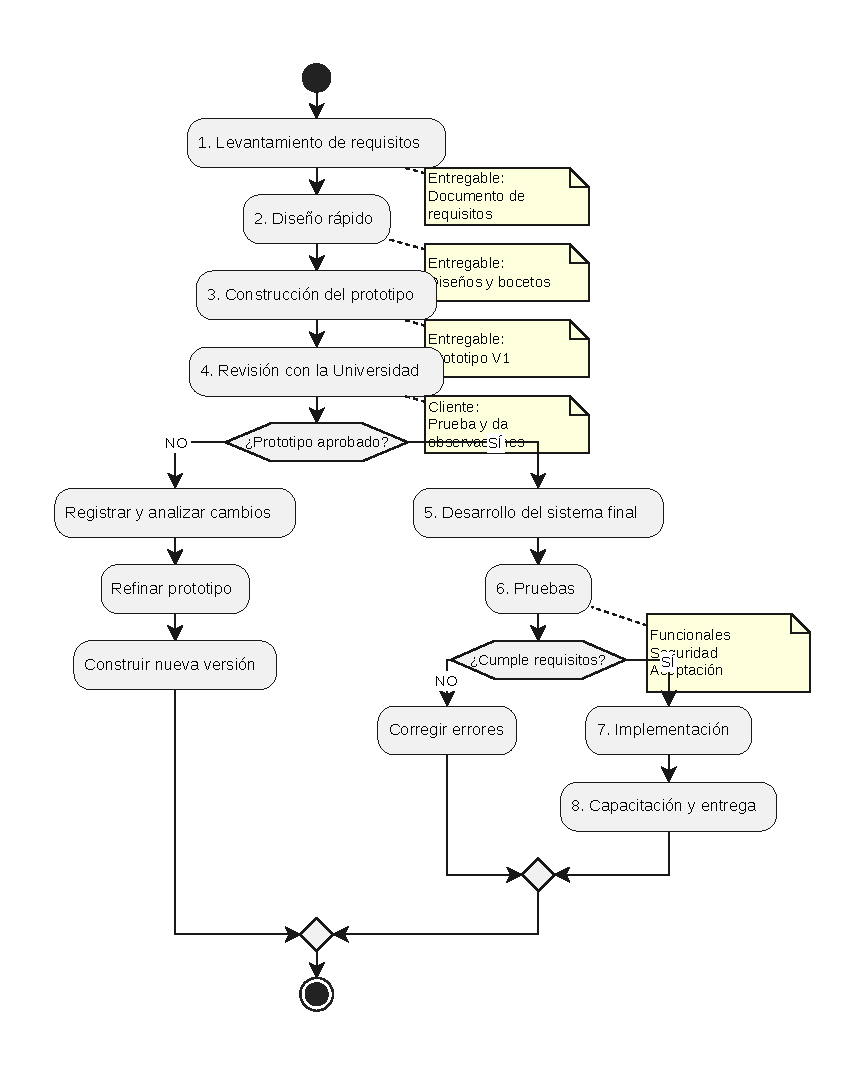
\includegraphics[width=0.8\textwidth]{TrabajoAguiles.drawio.pdf}
 	\caption{Flujo de trabajo del Modelo de Prototipos.}\label{fig:prototipos}
 \end{figure}
 
 \subsection{Parte 4: Evento Inesperado}
 % Responder las 7 preguntas guía de la Parte 4
 
 Al finalizar el tercer mes, la universidad solicita:
 
 \begin{itemize}
 	\item Aplicación móvil para docentes.
 	\item Reserva de laboratorios desde el celular.
 	\item Reporte de daños mediante fotografías.
 	\item Nuevas políticas de protección de datos.
 \end{itemize}
 
 
 \subsubsection{¿En qué fase se encuentra el proyecto?}
 
 Al finalizar el tercer mes, el proyecto se encuentra en la etapa de refinamiento y evaluación del prototipo, debido a que durante los tres primeros meses se han construido y revisado diferentes versiones.
 
 Por lo tanto, el cambio aparece en un momento en el que todavía se está trabajando con el prototipo y los requisitos están siendo validados. Esto es favorable para el Modelo de Prototipos, porque el nuevo requerimiento puede incorporarse como parte de una nueva iteración.
 
 
 \subsubsection{¿Qué documentos o productos deben modificarse?}
 
 Los principales documentos y productos que deberían modificarse son:
 
 \begin{itemize}
 	\item Requisitos funcionales.
 	\item Requisitos no funcionales.
 	\item Diseño del sistema.
 	\item Diseño de base de datos.
 	\item Prototipo.
 	\item Plan de pruebas.
 	\item Plan de seguridad.
 	\item Cronograma.
 	\item Presupuesto.
 \end{itemize}
 
 Además, deberán agregarse requisitos relacionados con la aplicación móvil y con la protección de datos.
 
 
 \subsubsection{¿Qué actividades tendrían que repetirse?}
 
 Al tratarse de un nuevo requerimiento importante, algunas actividades deberán repetirse:
 
 \begin{enumerate}
 	\item Levantamiento y análisis del nuevo requisito.
 	\item Revisión de requisitos existentes.
 	\item Diseño rápido de la aplicación móvil.
 	\item Diseño de la función para reportar daños mediante fotografías.
 	\item Revisión de las políticas de protección de datos.
 	\item Construcción de un nuevo prototipo.
 	\item Evaluación con docentes.
 	\item Recopilación de observaciones.
 	\item Refinamiento del prototipo.
 	\item Actualización de las pruebas.
 	\item Pruebas de seguridad y protección de datos.
 \end{enumerate}
 
 No sería necesario comenzar nuevamente todo el proyecto desde cero, porque el modelo permite continuar mediante una nueva iteración.
 
 
 \subsubsection{¿Cómo afectaría el cambio al tiempo y al costo?}
 
 \textbf{Tiempo:} aumentaría aproximadamente de 3 a 5 semanas.
 
 \textbf{Costo:} aumentaría por el desarrollo de la aplicación móvil, pruebas adicionales, almacenamiento de fotografías y aplicación de nuevas medidas de seguridad.
 
 
 \subsubsection{¿La metodología permite incorporar el cambio fácilmente?}
 
 Sí. Una de las principales ventajas del Modelo de Prototipos para este caso es que permite incorporar cambios durante las iteraciones.
 
 La universidad puede solicitar la nueva función, el equipo puede diseñar rápidamente una propuesta, construirla en el prototipo y presentarla nuevamente a los usuarios para obtener retroalimentación.
 
 Sin embargo, que sea flexible no significa que todos los cambios deban incorporarse inmediatamente. Se debe analizar su impacto antes de aprobarlos.
 
 El prototipado se caracteriza precisamente por la construcción de modelos que pueden ser evaluados y refinados con participación de los usuarios. Estudios académicos también reconocen el prototipado como una práctica utilizada para apoyar la ingeniería de requisitos y mejorar la comprensión de las necesidades del sistema.
 
 
 \subsubsection{¿Aceptaríamos el cambio inmediatamente, lo aplazaríamos o lo rechazaríamos?}
 
 En este caso aceptaríamos el cambio para su análisis, pero no comenzaríamos inmediatamente su desarrollo.
 
 Primero se realizaría un análisis de impacto para determinar:
 
 \begin{itemize}
 	\item Complejidad.
 	\item Tiempo adicional.
 	\item Costo adicional.
 	\item Riesgos.
 	\item Cambios en la arquitectura.
 	\item Cambios en la base de datos.
 	\item Requisitos de seguridad.
 	\item Recursos necesarios.
 \end{itemize}
 
 Después del análisis, si la universidad aprueba el nuevo tiempo y costo, se incorporaría el cambio en una nueva iteración del prototipo.
 
 Consideramos que rechazarlo directamente no sería conveniente porque se trata de una funcionalidad que puede aportar valor al sistema y, además, las nuevas políticas de protección de datos son importantes para el funcionamiento institucional.
 
 
 \subsubsection{Procedimiento formal para gestionar el cambio}
 
Se utilizará el siguiente procedimiento para gestionar los cambios solicitados durante el desarrollo del proyecto:

\begin{enumerate}
	\item \textbf{Solicitud de cambio:} La universidad registra formalmente la solicitud de incorporar la aplicación móvil y las nuevas políticas de protección de datos.
	
	\item \textbf{Análisis:} El equipo analiza los requisitos nuevos y determina qué partes del sistema serán afectadas.
	
	\item \textbf{Evaluación del impacto:} Se calcula el impacto en tiempo, costo, recursos, seguridad, arquitectura y pruebas.
	
	\item \textbf{Actualización de requisitos:} Si el cambio es viable, se actualizan los documentos de requisitos.
	
	\item \textbf{Aprobación:} La universidad y el responsable del proyecto aprueban formalmente el cambio.
	
	\item \textbf{Diseño rápido:} Se realiza un diseño inicial de la aplicación móvil y de las nuevas funcionalidades.
	
	\item \textbf{Construcción del prototipo:} Se desarrolla una nueva versión del prototipo incorporando la aplicación móvil.
	
	\item \textbf{Evaluación:} Los docentes y responsables prueban el prototipo y proporcionan observaciones.
\end{enumerate}
 
 %% =========================================================================
 %% SECCIÓN 2: METODOLOGÍA RAD (Pablo Toapanta)
 %% =========================================================================
 \section{Caso de Estudio: Metodología RAD}\label{sec:rad}
 \subsection{Parte 1: Análisis Inicial}
 \subsubsection{Identificación de Interesados}
 \subsubsection{Requisitos Funcionales (mínimo 8) y No Funcionales (4)}
 \subsubsection{Análisis de Riesgos (mínimo 3)}
 \subsubsection{Requisitos que Necesitan Mayor Aclaración}
 
 \subsection{Parte 2: Aplicación de la Metodología (Planificación a 6 Meses)}
\subsubsection{Justificación del modelo RAD}
La justificación de este modelo esta sustentada en la reestricción de tiempo de seis para la entrega del producto. La literatura científica demuestra que RAD es efectiva en escenarios dinamicos, donde se prioriza la velocidad y el prototipado iterativo \cite{purnamasari_rapid_2026}. 
De acuerdo a la literatura consultada en \cite{purnamasari_rapid_2026} y \cite{alvarez-pineda_implementacion_2026} las fases de la metodologia RAD son:
\begin{itemize}
	\item \textbf{Planificacion de requisitos}. En esta fase se definen de manera supercifial los requerimeintos esenciales  a través de entrevistas semiestructuradas y talleres de Diseño Conjunto de Aplicaciones con los skateholders.
	\item \textbf{Diseño de usuario}. En esta fase se usan maquetas de alta fidelidad, con el fin de ejecutar varios ciclos de retroalimentacioin donde los usuarios interactuen con la interfaz para validad la navegacion y estructura de la aplicacion.
	\item \textbf{Construccion}. En esta fase se empieza a codificar todos los modulos que componen el sistema, siempre haciendo pruebas tempranamente para asegurar correcta funcionalidad.
	\item \textbf{Transicion}. En esta fase se valida el entorno de produccion real, se capacitan a los usuarios y se pone en marcha a la aplicacion.
\end{itemize}
 \subsubsection{Fases RAD }
En la adaptación práctica del proyecto universitario, estas fases se correlacionan de la siguiente manera \cite{purnamasari_rapid_2026}:
\begin{enumerate}
	\item \textbf{Modelado de Gestión y Datos (Planificación):} Identificación de la información que fluye entre los responsables de laboratorio y docentes. Mapeo de inventario (equipos) y usuarios.
	\item \textbf{Modelado de Proceso (Diseño de Usuario):} Definición de cómo la información se transforma (flujo de reserva, check-in/check-out de equipos). Se materializa en prototipos.
	\item \textbf{Generación de la Aplicación (Construcción):} Uso de herramientas de desarrollo rápido, frameworks o herramientas Low-Code/RAD \cite{radvilaite_integrating_2025} para transformar los diseños en código ejecutable.
	\item \textbf{Pruebas y Entrega (Transición):} Comprobación del sistema integrado, pruebas de usabilidad y despliegue final.
\end{enumerate}
 
 \subsubsection{Productos y Entregables por Fase}
 \begin{itemize}
 	\item \textbf{Fase 1:} Matriz de Requisitos (SRS), Diagrama de Casos de Uso y Cronograma inicial \cite{purnamasari_rapid_2026}.
 	\item \textbf{Fase 2:} Prototipos navegables (UI/UX en Figma), Modelo Entidad-Relación y diagramas de actividad \cite{alvarez-pineda_implementacion_2026, purnamasari_rapid_2026}.
 	\item \textbf{Fase 3:} Código fuente funcional versionado, Base de datos integrada.
 	\item \textbf{Fase 4:} Manuales de usuario, Reporte de Pruebas de Aceptación (UAT) y Sistema en Producción \cite{purnamasari_rapid_2026}.
 \end{itemize}
 \subsubsection{Matriz de Responsables y Equipos Paralelos}
 La metodología RAD sugiere dividir el desarrollo en equipos paralelos para ganar velocidad \cite{purnamasari_rapid_2026}:
 \begin{itemize}
 	\item \textbf{Equipo A (Gestión y Usuarios):} Desarrolladores y Analistas encargados del catálogo de laboratorios y control de roles.
 	\item \textbf{Equipo B (Reservas y Préstamos):} Desarrolladores encargados del motor de reservas, reportes de daños y check-in/out.
 	\item \textbf{Responsables Transversales:} Diseñador UI/UX, QA Tester, Administrador de Base de Datos y los Stakeholders (Docentes/Encargados de laboratorio) que participan continuamente.
 \end{itemize}
 \subsubsection{Estrategia de Pruebas y Control de Calidad}
La estrategia de aseguramiento de calidad será continua y se integrará dentro de los ciclos iterativos de RAD, empleando las siguientes técnicas documentadas en la literatura \cite{purnamasari_rapid_2026, alvarez-pineda_implementacion_2026}:

\begin{itemize}
	\item \textbf{Pruebas de Caja Gris (Grey-Box Testing):} Implementadas durante la fase de Construcción. De acuerdo con la metodología aplicada en \cite{purnamasari_rapid_2026}, estas pruebas combinan el análisis funcional (caja negra) con la validación de la estructura interna del código (caja blanca). En este proyecto, son cruciales para verificar las interacciones complejas en la base de datos (por ejemplo, asegurar que cuando un equipo tecnológico se reserva, el stock disminuya correctamente en el \textit{backend}) mientras se prueba la interfaz.
	
	\item \textbf{Pruebas de Accesibilidad y Usabilidad:} Ejecutadas iterativamente sobre los prototipos. Se evaluará el contraste de colores, etiquetas descriptivas y la correcta jerarquía visual de los formularios de reserva, garantizando una navegación accesible e intuitiva \cite{alvarez-pineda_implementacion_2026}.
	
	\item \textbf{Pruebas de Aceptación del Usuario (UAT):} Ejecutadas en la fase de Transición. Consisten en pruebas prácticas donde los distintos roles (Administrador, Docente, Estudiante) validan el sistema bajo escenarios de trabajo reales (como generar un reporte mensual o aprobar un préstamo) para confirmar que cumple con todos los requisitos \cite{purnamasari_rapid_2026}.
\end{itemize}
\subsubsection{Mecanismo de Gestión de Cambios (Cajas de Tiempo e Implementación por Fases)}
Siguiendo las directrices de la metodología RAD, el tiempo de entrega de 6 meses es inamovible. Para gestionar los cambios o nuevos requerimientos, se utilizará la técnica de \textit{Timeboxing} en iteraciones estrictas \cite[p.~340]{purnamasari_rapid_2026}. Además, si una funcionalidad solicitada (como un cambio de alcance) excede el tiempo de desarrollo asignado, se aplicará un enfoque de implementación por fases: las funciones críticas se desplegarán primero para cumplir con el plazo, y las características secundarias se postergarán para actualizaciones futuras \cite[p.~340]{purnamasari_rapid_2026}.
 \subsubsection{Cronograma General a 6 Meses}
 \begin{itemize}
 	\item \textbf{Mes 1:} Planificación de requisitos (Entrevistas y definición de alcance).
 	\item \textbf{Mes 2 al Mes 3 (15 días):} Diseño de usuario (Wireframes, validación iterativa).
 	\item \textbf{Mes 3 (15 días) al Mes 5:} Construcción modular rápida (Equipos A y B en paralelo) y pruebas unitarias.
 	\item \textbf{Mes 6:} Transición (Migración de datos, Pruebas de Aceptación de Usuarios, capacitación y despliegue final).
 \end{itemize}
 
 \subsection{Parte 3: Representación Visual}
 % Insertar diagrama de draw.io
  \begin{figure}[htbp]
 	 \centering 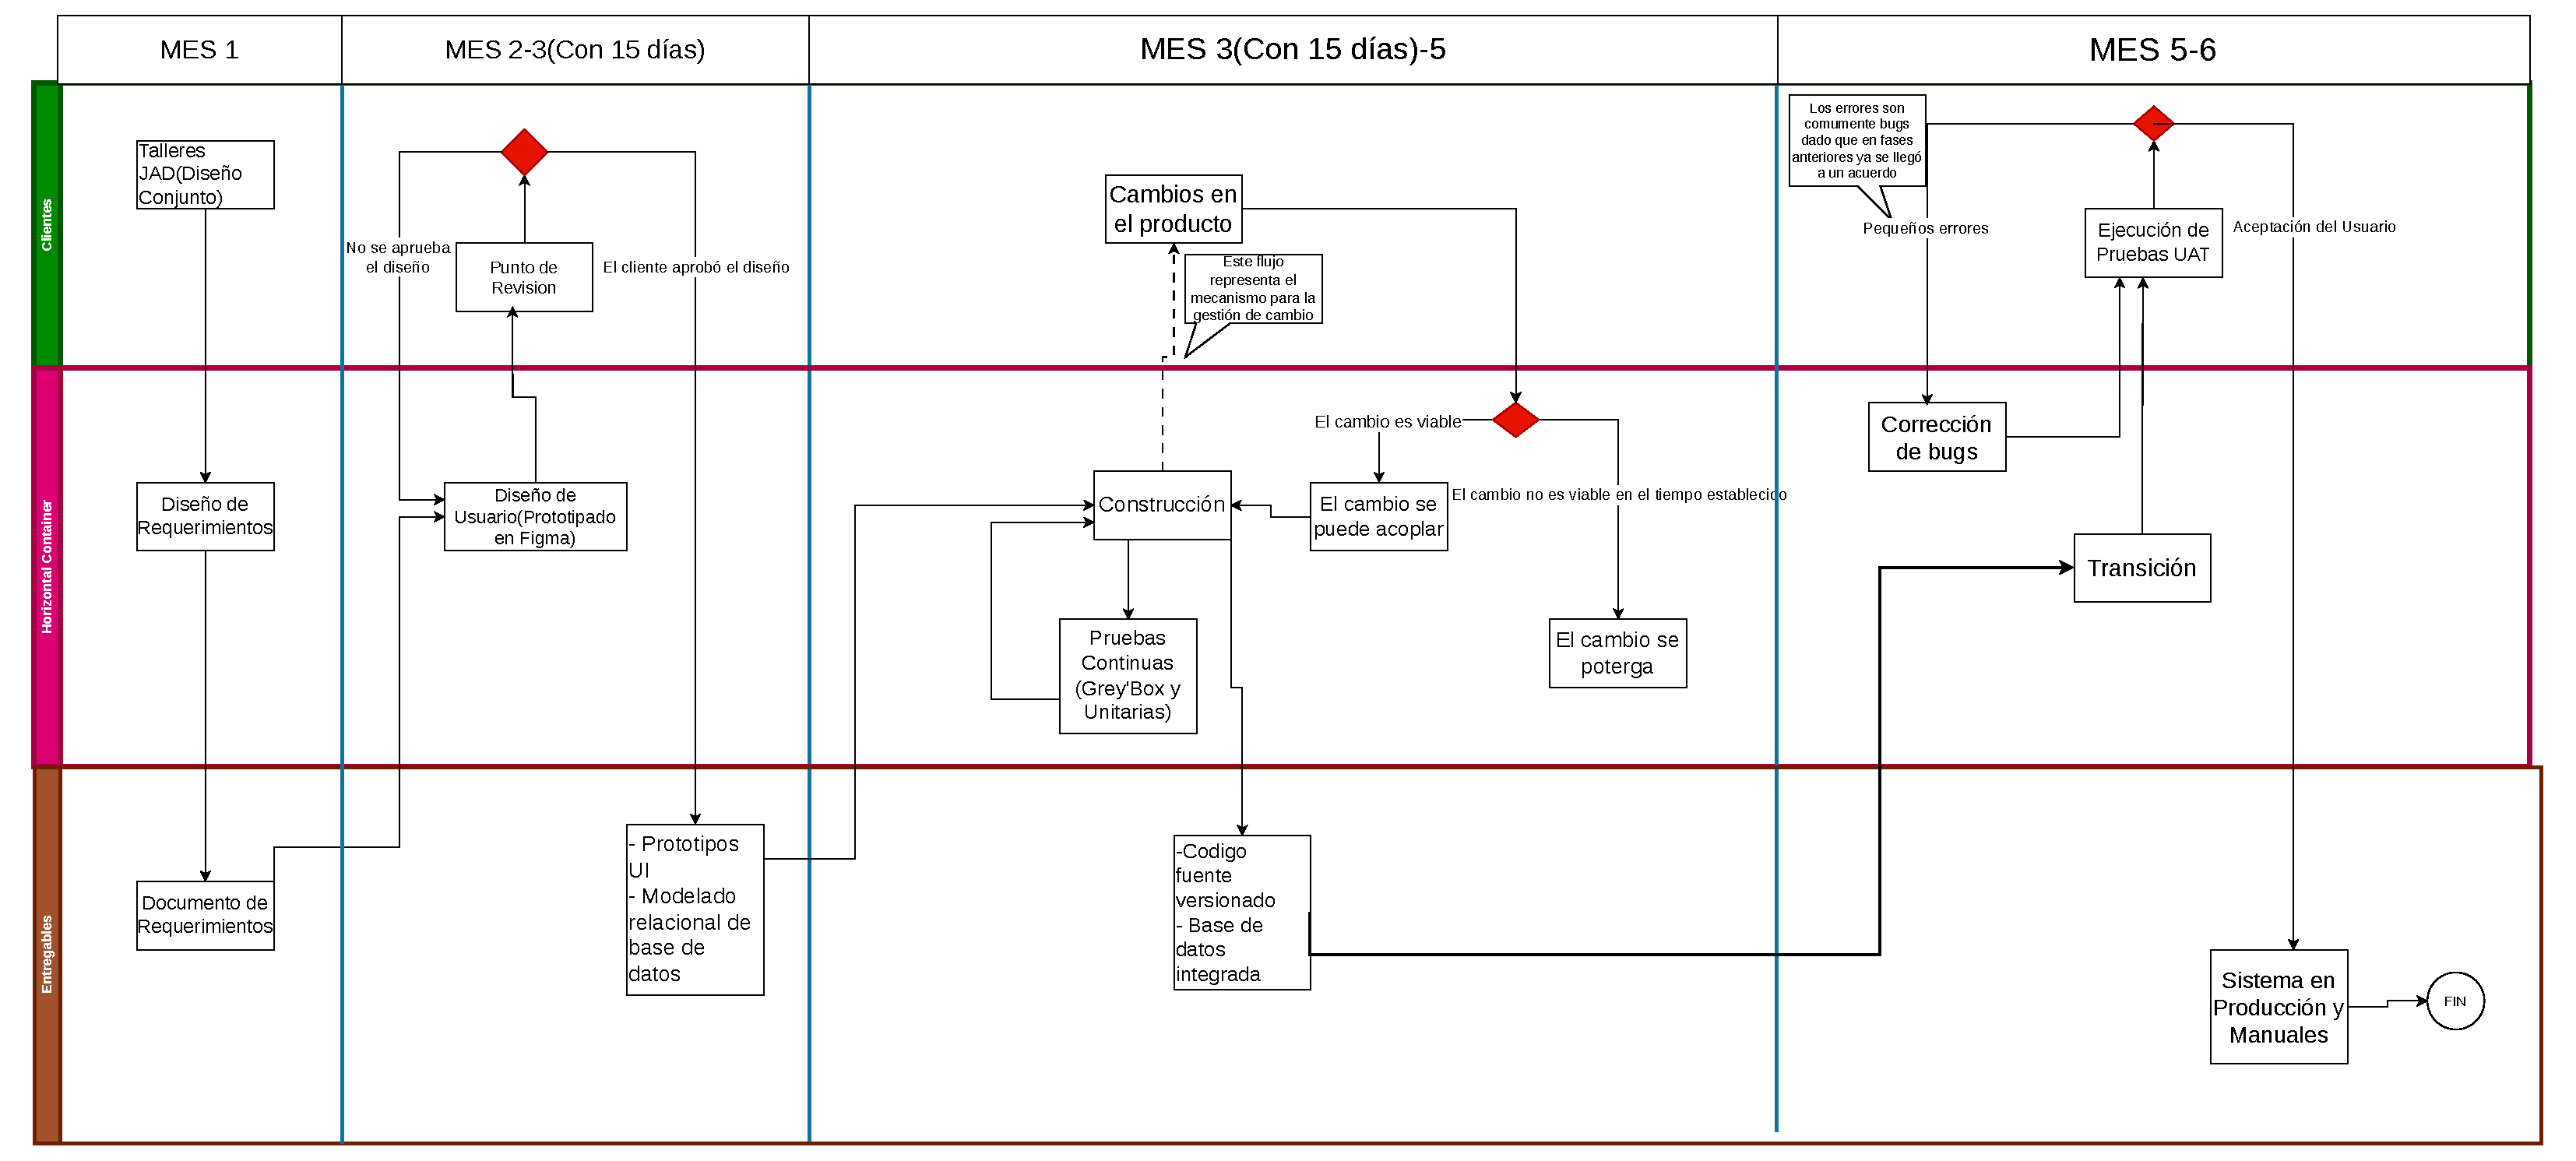
\includegraphics[width=0.8\textwidth]{DiagramaDeberAgiles.drawio.pdf}
 	\caption{Flujo de trabajo de la Metodología RAD.}\label{fig:rad}
 	 \end{figure}
 
 \subsection{Parte 4: Evento Inesperado (App Móvil y Protección de Datos)}
 % Responder las 7 preguntas guía de la Parte 4
 
 %% =========================================================================
 %% SECCIÓN 3: PREGUNTAS DE DISCUSIÓN FINAL (Individual / Comparativa)
 %% =========================================================================
 \section{Preguntas para la Discusión Final}\label{sec:discusion}
 \subsection{Perspectiva desde el Modelo de Prototipos (Leslie Coello)}
 \subsection{Perspectiva desde la Metodología RAD (Pablo Toapanta)}
 
 %% =========================================================================
 %% SECCIÓN 4: PRESENTACIÓN, DEFENSA Y CONCLUSIÓN
 %% =========================================================================
 \section{Presentación y Defensa}\label{sec:defensa}
 \textbf{Enlace de sustentación en YouTube (3-4 minutos):} \url{https://youtube.com/...}
 
 \subsection{Conclusión Argumentada de Idoneidad}
 
 

%%=============================================%%
%% For submissions to Nature Portfolio Journals %%
%% please use the heading ``Extended Data''.   %%
%%=============================================%%

%%=============================================================%%
%% Sample for another appendix section			       %%
%%=============================================================%%

%% \section{Example of another appendix section}\label{secA2}%
%% Appendices may be used for helpful, supporting or essential material that would otherwise 
%% clutter, break up or be distracting to the text. Appendices can consist of sections, figures, 
%% tables and equations etc.



%%===========================================================================================%%
%% If you are submitting to one of the Nature Portfolio journals, using the eJP submission   %%
%% system, please include the references within the manuscript file itself. You may do this  %%
%% by copying the reference list from your .bbl file, paste it into the main manuscript .tex %%
%% file, and delete the associated \verb+\bibliography+ commands.                            %%
%%===========================================================================================%%

\bibliography{sn-bibliography}% common bib file
%% if required, the content of .bbl file can be included here once bbl is generated
%%\input sn-article.bbl
\begin{thebibliography}{9}
	
	\bibitem{iso2018}
	International Organization for Standardization (ISO). (2018). \textit{ISO/IEC/IEEE 29148:2018 -- Systems and software engineering -- Life cycle processes -- Requirements engineering}. ISO.
	
	\bibitem{wood1992}
	Wood, D.~P., \& Kang, K.~C. (1992). \textit{A Classification and Bibliography of Software Prototyping}. Software Engineering Institute, Carnegie Mellon University.
	
	\bibitem{openstax}
	OpenStax / Rice University. \textit{Software Engineering Process}. Engineering LibreTexts.
	
	\bibitem{mumbai}
	University of Mumbai. \textit{Software Engineering and Project Management}.
	
	\bibitem{bjarnason2023}
	Bjarnason, E., Lang, F., \& Mj\"oberg, A. (2023). An empirically based model of software prototyping: a mapping study and a multi-case study. \textit{Empirical Software Engineering}, 28, 115.
	
\end{thebibliography}

\end{document}
